% Copyright 2025 Kieran W Harvie. All rights reserved.

\section{Monotone Bézier Curve}
A curve is called monotone with respect an axis if every line perpendicular to the axis crosses the curve at most once.\footnote{
Not to be confused with a polygon being called monotone with respect an axis if every line perpendicular to the axis crosses the polygon at most twice.
This is because for every axis and non-degenerate closed curve there exits a perpendicular line that crosses the closed curve at least twice making the original curve definition useless.}
\begin{center}
\begin{tikzpicture}
	\draw (0,0) .. controls (10,0) and (-2,4) ..  (8,4);
	\draw[red,dashed] (4,0) --  (4,4);
\end{tikzpicture}

A cubic Bézier curve failing to be monotone with the horizontal axis.
\end{center}
For another project I wanted confirmation that cubic Bézier curves with control points:
\[\mathbf{P}_0=(0,0)\quad\mathbf{P}_1=(1-k,0)\quad\mathbf{P}_2=(k,1)\quad\mathbf{P}_3=(1,1)\]
Are monotone with the horizontal axis when $k\in[0,\frac{1}{2}]$,
as they certainly look monotonous:
\begin{center}
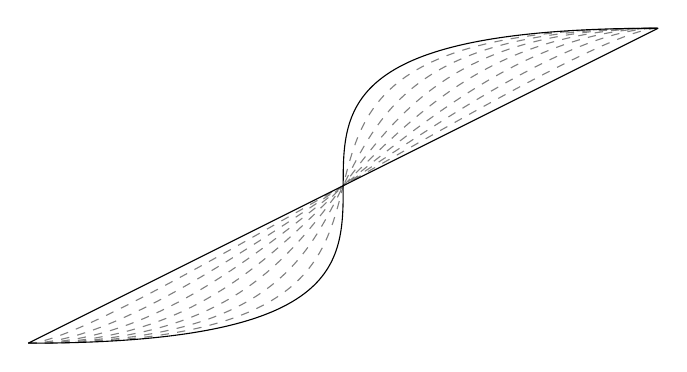
\begin{tikzpicture}
	\foreach \i in {1,...,7}
	\draw[gray, dashed] (0,0) .. controls (8-\i,0) and (\i,4) ..  (8,4);

	\draw (0,0) -- (8,4)
		(0,0) .. controls (8,0) and (0,4) ..  (8,4);
\end{tikzpicture}
\end{center}
Originally I tried to prove this by projecting the curve onto the $x$-axis and then using standard algebraic methods.
But midway through I realized that the result is trivial when applying the variation diminishing property of Bézier curves.
I've included both methods as I'd done most of the work already and it might still be useful.

\subsection{Diminishing Variation}
The variation diminishing property of Bézier curves is quite simple.
The number of times a line intersects a Bézier curve is less than or equal to the times it intersects the chain formed by the curves control points.
When $k\in (0,\frac{1}{2})$ none of the chain's segments are vertical or measurably overlap each other on the $x$-axis.
Hence the chain is intersected at most once by any vertical line,
meaning so is the curve.
\\

When $k=0$ the curve is a simple line and monotony is trivial.
When $k=\frac{1}{2}$ we have a problem that the $(1-k,0)$ to $(k,1)$ segment is a vertical line.
This can be removed with a single degree elevation:
\[\mathbf{P}_0 = (0,0),\mathbf{P}_1 = \left(\tfrac{3}{4}(1-k),0\right),\mathbf{P}_2 = \left(\tfrac{1}{2},\tfrac{1}{2}\right),\mathbf{P}_3=\left(\tfrac{1}{4}(1+3k),1\right),\mathbf{P}_4=(1,1)\]
\begin{center}
\begin{tikzpicture}
	\draw (0,0) .. controls (8,0) and (0,4) ..  (8,4);
	\draw[red] (0,0) -- (3,0)--(4,2)--(5,4)--(8,4);
	\fill[red] (0,0) circle (2pt) -- (3,0) circle (2pt)--(4,2) circle (2pt) -- (5,4) circle (2pt)--(8,4) circle (2pt);
\end{tikzpicture}

The $k=\frac{1}{2}$ case with the degree elevated control polygon shown.
\end{center}
(Note that we could have degree elevated from the beginning,
but it felt excessive for the general case.)

\subsection{Projection}
The following expression is for the projection of a Bézier curve on the $\hat{\mathbf{a}}$ axis:
\[A(t) = \hat{\mathbf{a}}\cdot\left((1-t)^3\mathbf{P}_0+3t(1-t)^2\mathbf{P}_1(1-t)\mathbf{P}_2+t^3\mathbf{P}_3\right)\]
The resulting function is a polynomial, a very well behaved function.
\\

To prove a curve is monotone it is sufficient to show that the function's derivative is always non-negative or always non-positive and $A(t)$'s  derivative is simply a parabola:
\[\dot{A}(t) = A_0(1-t)^2+2A_1t(1-t)+A_2t^2\]
With coefficients:
\[A_n = 3\hat{\mathbf{a}}\cdot\left(\mathbf{P}_{n+1}-\mathbf{P}_n\right)\]
Where $A_n$ is the displacement of $P_{n+1}$ from $P_{n}$ along the $3\hat{\mathbf{a}}$ axis.

\subsubsection{Determinant:}
The first attempt to solve this problem is to consider the determinant of $\dot{A}(t)$,
there's a problem with this method.
We only care about a sign change in $t\in[0,1]$,
meaning we could have a positive determinant and still have a monotone curve.
So if we got a positive determinant we would need to calculate the roots and check that they are both outside $t\in[0,1]$.
This isn't to hard for a computer,
and may be the best option for handling arbitrary curves and axises,
but it is needlessly involved if we just want a simple proof of monotony for a known family of curves.
\\

Since it might be useful for computation we can write $\dot{A}(t)$ in pretty direct terms of $\mathbf{P}_n$ as:
\[\dot{A}(t) = (a_3-3a_2+3a_1-a_0)t^2+2(a_2-2a_1+a_0)t+(a_1-a_0)\]
Where:
\[a_n = 3\hat{\mathbf{a}}\cdot\mathbf{P}_n\]

\subsubsection{Checking Signs:}
Note that all of $(1-t)^2$, $2t(1-t)$, and $t^2$ are nonnegative when $t\in[0,1]$.
Furthermore,
that at least one of them is non-zero at any point in the domain.
Hence if $A_n$ are all non-zero and share the same sign then $\dot{A}(t)$ has no roots.
This is intuitive as it correspond to all of $\mathbf{P}_n$ moving in the same direction along the $\hat{\mathbf{a}}$ axis.

\subsubsection{Flip the Sign of $A_1$:}
Consider the following relation:
\[(2t-1)^2 = (t-(1-t))^2= (1-t)^2-2t(1-t)+t^2\]
Applying this to $\dot{A}(t)$ we can remove the $2t(1-t)$ term:
\[\begin{aligned}
	\dot{A}(t) =& A_0(1-t)^2+2A_1t(1-t)+A_2t^2\\
	=&(A_0+A_1)(1-t)^2+(A_2+A_1)t^2-A_1(2t-1)^2\\
\end{aligned}\]
Observe that all of $t^2$, $(1-t)^2$, and $(2t-1)^2$ are positive.
So,
similar to before,
$A(t)$ is monotone if all of $A_0+A_1$, $A_1+A_2$ and $-A_1$ have the same sign.
In essence we can flip the sign of $A_1$ by also adding it to $A_0$ and $A_2$.
\\

Geometrically,
this means $\mathbf{P}_n$ can change the direction they're going along the $\hat{\mathbf{a}}$ axis provided the move from $\mathbf{P}_0$ to $\mathbf{P}_1$ and from $\mathbf{P}_2$ to $\mathbf{P}_3$ is larger in magnitude then from $\mathbf{P}_1$ to $\mathbf{P}_2$.

% I'm not sure what this is but not deleting it for now.
% Even though I think the first equation is wrong.
%
%\subsubsection{Dealing with Edge cases:}
%\[\dot{A}(t) = 3((1-t)^2+2t(1-t)(2k-1)+t^2(1-k)) = 3((1-k)(2t-1)^2+k2t(1-t))\]
%\[\begin{aligned}
%	\dot{A}(t) =& 3((1-k)(1-t)^2+2t(1-t)(2k-1)+t^2(1-k))\\
%	=& 3(1-k)((1-t)^2+2t(1-t)+t^2)+6(3k-2)t(1-t)\\
%\end{aligned}\]
